\documentclass[12pt]{article}
	
%______________________PREAMBULO_________________________

%----------------------Paquetes--------------------------
\usepackage{amsmath,amssymb,amsfonts,latexsym,cancel} % Paquetes de símbolos adicionales.
\usepackage[spanish,es-tabla]{babel} % Idioma español
\usepackage[utf8]{inputenc} % Paquete que nos permite usar los acentos y otros símbolos, directamente del teclado.
\usepackage[T1]{fontenc} % Cambia el tipo de letra
\usepackage{times} % Tipo de letra Times New Roman
\usepackage{graphicx} % Paquete para el manejo de gráficos y figuras en el documento.
\usepackage{geometry} % Permite el manejo de los margenes
\usepackage{fancyhdr} % Permite colocar y manejar el encabezado
\usepackage[breaklinks,colorlinks=true,linkcolor=black,citecolor=blue, urlcolor=blue]{hyperref} % Crea hipervinculo entre secciones y el indice
\usepackage{pstricks}
\usepackage{multicol}
%\usepackage{mathpazo} %fuente palatino
%\usepackage{xcolor}
%\usepackage[shortlabels]{enumitem}
%-------------Paquetes para el formato de las citas-------
%\usepackage[hyphens]{url}
%\usepackage{float}
%\usepackage{cite}
%\usepackage{wrapfig}

%-----------------------------ayuda de paquetes--------------------

\spanishdecimal{.}

%------------------------Margenes----------------------------

\newgeometry{bottom = 2.5 cm, top = 2.5 cm, left = 2 cm, right = 2 cm} % Modifica el margen {Abajo, Arriba, Izquierda, Derecha

%----------------------------Interlineado----------------------------------

%\doublespacing
%\onehalfspace
%\singlespace
%\spacing{1.5} % Permite personalisar a gusto
%\setlength{\parskip}{2cm} % Es el espacio entre parrafos

%-----------------------------Sangria---------------------------------------

\setlength{\parindent}{0 cm} % Manipula la sangria

%---------------------Portada------------------

%\title{
%\begin{figure}[h!]
		
%	\centering
%	
\includegraphics[width=\linewidth]{Nom_UAdeC_FCFM.png}  			
			
%\end{figure}
%\huge \textbf{LABORATORIO DE FISICA 3}\\\LARGE TITULO PRACTICA\\}
%\author{ \Large \textbf{Profesor:}\\
%\Large \textbf{Alumno:} Oscar Joel Castro Contreras}
%\date{\today}

%--------------Encabezado y pie de pagina--------------------

\pagestyle{fancy}%Coloca el encabezado en el documento
\lhead[]{Métodos numéricos}%Encabezado izquierda
\rhead[]{Oscar Joel Castro Contreras}%Encabesado derecha
%\chead[]{}%Encabesado central
\renewcommand{\headrulewidth}{0.08 pt}%Coloca linea al pie de pagina

%\lfoot[]{PI}%Pie de pagina izquerdo
%\rfoot[]{PD}%Pie de pagina derecho
\cfoot[]{\thepage}%Pie de pagina central
\renewcommand{\footrulewidth}{0.08 pt}%Coloca linea al pie de pagina

%-----------------------------------------------------------------------------

	\begin{document}
		
		\begin{titlepage}
		
			\centering
			{\bfseries
			\begin{figure}[h!]
				\centering
				
\includegraphics[width=\linewidth]{Nom_UAdeC_FCFM.png} 				
			\end{figure}
			\par}
			\vspace{2cm}
			{\scshape\LARGE Métodos numéricos \par}
			\vspace{3cm}
			{\scshape\Huge \textbf{Mínimos Cuadrados} \par}
			\vfill
			{\LARGE \textbf{Profesora:} Maria Guadalupe Godina Cubillo \par}
			\vspace{3cm}
			{\LARGE \textbf{Alumno:} Oscar Joel Castro Contreras \par}
			\vfill
			{\Large \today \par}
			\thispagestyle{empty}
			%\thispagestyle{fancy}
			
		\end{titlepage}
	
		\newpage

		\begin{abstract}
			\noindent En este reporte explico como se aplica el método de mínimos cuadrados 
			en un conjunto de datos para obtener una recta que se ajuste a estos datos.
		\end{abstract}

		\textbf{Palabras clave:} Minimos Cuadrados, Recta.

		\section*{\centering Introducción}\label{sec:Introducción}
			Es un procedimiento de análisis numérico en la que, dados un conjunto de puntos, se intenta 
			determinar la función continua que mejor se aproxime a los datos, proporcionando una demostración 
			visual de la relación entre los puntos de estos. En su forma más simple, busca minimizar la 
			suma de cuadrados de las diferencias ordenadas entre los puntos generados por la función y los 
			correspondientes datos. \cite{bib:item1}\\
			El método de mínimos cuadrados consiste es una técnica de optimización cuyo objetivo consiste 
			en la obtención de la función que mejor se ajuste, en el sentido de un error cuadrático mínimo 
			a los datos observados de las variables objeto de estudio. \cite{bib:item2}\\
			La creación del método de mínimos cuadrados generalmente se le acredita al matemático alemán Carl 
			Friedrich Gauss, quien lo planteó en 1794 pero no lo publicó sino hasta 1809. El matemático francés 
			Andrien-Marie Legendre fue el primero en publicarlo en 1805, este lo desarrolló de forma independiente.\\
			Este método se utiliza comúnmente para analizar una serie de datos que se obtengan de algún estudio, 
			con el fin de expresar su comportamiento de manera lineal y así minimizar los errores de la data 
			tomada. \cite{bib:item1}
		
		\section*{\centering Metodología}\label{sec:Metodologia}
			El enfoque de mínimos cuadrados para este problema implica determinar la mejor línea de aproximación 
			cuando el error relacionado es la suma de los cuadrados de las diferencias entre los valores y en la 
			línea de aproximación y los valores y proporcionados. Por lo tanto, deben encontrarse las constantes 
			$ a_0 $ y $ a_1 $ que minimizan el error de mínimos cuadrados:
			$$ E_2(a_0,a_1) = \sum_{i=1}^{10}[y_i - (a_1x_i + a_0)]^2 $$
			El método de mínimos cuadrados es el procedimiento más conveniente para determinar mejores aproximaciones 
			lineales, pero también hay consideraciones teóricas importantes que lo favorecen. En general, mientras 
			el enfoque en los mínimos y máximos asigna demasiado peso a un bit de datos con un gran error, 
			el método de desviación absoluta no da suficiente peso a un punto que está fuera de la línea con la 
			aproximación. El enfoque de mínimos cuadrados asigna considerablemente más peso en un punto que está 
			fuera de la línea que al resto de los datos, pero no permitirá que el punto domine por completo la 
			aproximación. Una razón adicional para considerar el enfoque de mínimos cuadrados implica el estudio 
			de la distribución estadística del error.\\
			El problema general de ajustar la mejor línea de mínimos cuadrados para una recopilación de datos 
			$ \{(xi,yi)\}^m_{i=1} $ implica minimizar el error total.
			$$ E = E_2(a_0,a_1) = \sum_{i=1}^{m}[y_i - (a_1x_i + a_0)]^2 $$
			respecto a los parámetros $ a_0 $ y $ a_1 $. Para que se presente un mínimo, necesitamos que la derivada parcial 
			del error respecto a estos parámetros sea cero:
			$$ \frac{\partial E}{\partial a_0} = 0 \qquad \frac{\partial E}{\partial a_1} = 0, $$
			es decir
			$$ 0 = \frac{\partial}{\partial a_0} \sum_{i=1}^{m}[y_i - (a_1x_i + a_0)]^2 $$
			y
			$$ 0 = \frac{\partial}{\partial a_1} \sum_{i=1}^{m}[y_i - (a_1x_i + a_0)]^2. $$
			Estas ecuaciones se simplifican en las ecuaciones normales:
			$$ a_0 m + a_1 \sum_{i=1}^{m} x_i = \sum_{i=1}^{m} y_i $$
			y
			$$ a_0 \sum_{i=1}^{m} x_i + a_1 \sum_{i=1}^{m} x_i^2 = \sum_{i=1}^{m} x_iy_i. $$
			La solución para este sistema de ecuaciones es:
			$$ a_0 = \frac{\displaystyle \sum_{i=1}^{m} x_i^2 \sum_{i=1}^{m} y_i - \sum_{i=1}^{m} x_iy_i \sum_{i=1}^{m} x_i}{\displaystyle m\left( \sum_{i=1}^{m} x_i^2 \right) - \left( \sum_{i=1}^{m} x_i \right)^2} $$
			y
			$$ a_1 = \frac{\displaystyle m\sum_{i=1}^{m} x_iy_i - \sum_{i=1}^{m} x_i \sum_{i=1}^{m} y_i}{\displaystyle m\left( \sum_{i=1}^{m} x_i^2 \right) - \left( \sum_{i=1}^{m} x_i \right)^2} $$
			con estos parámetros podemos encontrar la recta que se ajuste a los datos de la forma:
			$$ a_1x + a_0 $$
			\cite{bib:item3}
			\newpage

		\section*{\centering Resultado}\label{sec:Resultado}
			Por ejemplo tenemos esta tabla de datos $ (x_i, y_i) $ de la cual podemos obtener un 
			aproximación a una recta usando lo antes explicado: \\
			\begin{table}[h!]
				\centering
				\begin{tabular}{|c    c    c    c    c    c    c    c    c    c    c|}
					\hline
					$ x_i $ & 1 & 2 & 3 & 4 & 5 & 6 & 7 & 8 & 9 & 10 \\\hline
					$ y_i $ & 1.3 & 3.5 & 4.2 & 5.0 & 7.0 & 8.8 & 10.1 & 12.5 & 13 & 15.6 \\\hline							
				\end{tabular}
				\caption{Datos $ (x_i, y_i) $ para aproximar a una recta .\cite{bib:item3}}
				\label{tab:1}
			\end{table}\\
			Para ayudarnos de otra tabla como la tabla \ref{tab:2} para calcular primero de $ x_iy_i $ y $ x_i^2 $, 
			después sumamos las columnas para obtener las sumatoria: \\
			\begin{table}[h!]
				\centering
				\begin{tabular}{c    c    c    c    c    c}
					\hline
					& $ x_i $ & $ y_i $ & $ x_iy_i $ & $ x_i^2 $ \\\hline
					& 1 & 1.3 & 1.3 & 1 \\							
					& 2 & 3.5 & 7.0 & 4 \\
					& 3 & 4.2 & 12.6 & 9 \\
					& 4 & 5.0 & 20.0 & 16 \\
					& 5 & 7.0 & 35.0 & 25 \\
					& 6 & 8.8 & 52.8 & 36 \\
					& 7 & 10.1 & 70.7 & 49 \\
					& 8 & 12.5 & 100.0 & 64 \\
					& 9 & 13.0 & 117.0 & 81 \\
					& 10 & 15.6 & 156.0 & 100 \\\hline
					$ \sum = $& 55 & 81.0 & 572.4 & 385 \\\hline
				\end{tabular}
				\caption{Obtención de $ x_iy_i $ y $x_i^2 $ y su sumatoria.\cite{bib:item3}}
				\label{tab:2}
			\end{table}\\
			Ahora solo no que da obtener los parámetros para encontrar la recta, con las formulas antes mostradas:
			$$ a_0 = \frac{385(81) - 55(572.4)}{10(385) - (55)^2} = -0.360 $$
			y
			$$ a_1 = \frac{10(572.4) - 55(81)}{10(385) - (55)^2} = 1.538 $$
			Por lo que la ecuación de la recta es:
			$$ 1.538x - 0.360 $$
			Ahora para comprobar esto, mi programa sigue el mismo procedimiento mostrado por lo que podemos calcular 
			si meto los datos de la tabla \ref{tab:1} mi programa me da lo que se puede ver en la figura 1.
			\begin{center}
				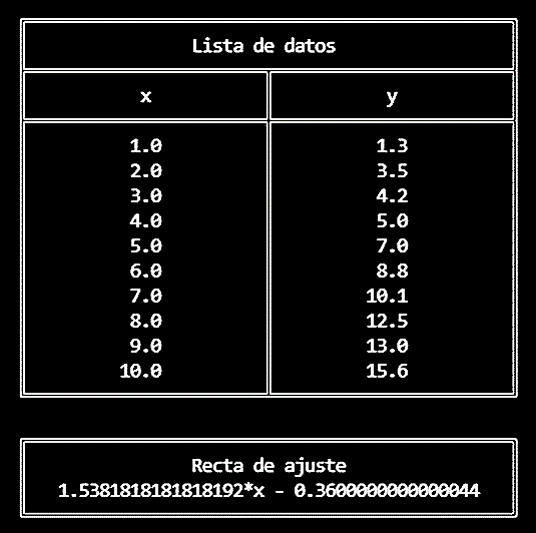
\includegraphics[width=.5\linewidth]{Figura 1.png}\\
				Figura 1: Función de la recta que arroja mi programa.
				\label{Fig:1}
			\end{center}
			Mi programa también tiene la opción de graficar por lo que si le pido la grafica a mi programa me arroja 
			lo grafica 1.
			\begin{center}
				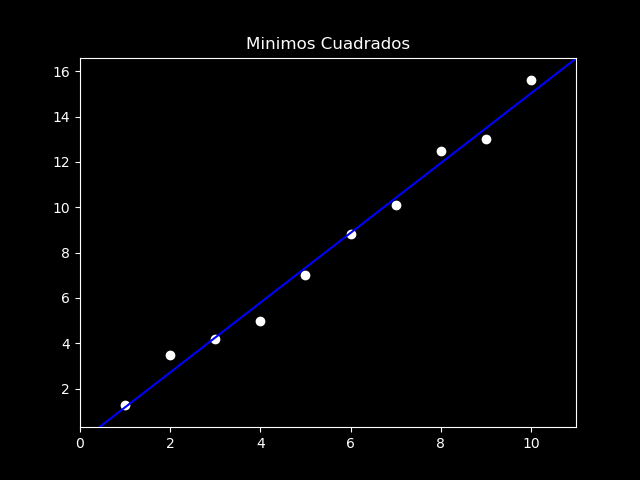
\includegraphics[width=.85\linewidth]{Grafica 1.png}\\
				Grafica 1: Grafica de los datos y la recta que arroja mi programa.
			\end{center}

		\section*{\centering Observación}\label{sec:Observacion}
			Como ya vimos este método es muy sencillo de aplicar, a cualquier conjunto de datos, en lo que yo lo 
			estuve probando con distritos datos no encontré ninguna restricción que impidiera crear la recta. Veo 
			que puede ser muy útil para ver la tendencia que tiene los datos, si tienden a bajar o a subir, esta 
			recta se puede usar mucho en estadística, ya que lo que hace es, al sumar el error de los puntos calcula 
			la recta por la que ese error sumado es el más pequeño posible.
		\section*{\centering Conclusión}\label{sec:Conclusion}
			El método toma el error de los datos dados y con ellos obtiene los parámetros para poder crear una recta 
			que cruce por la parte donde al sumar el error de cada dato, este sea el más pequeño. Podemos verlo como 
			una recta que esta siendo jalada por el error de cada uno de los datos y cuando la recta queda 
			en equilibrio es cuando al sumar el error de todos los datos es el mas pequeño y hay es donde se coloca la 
			recta. Esta recta es la que se crea con el metodo de minimos cuadrados.

		\centering
		\begin{thebibliography}{10}
			\bibitem{bib:item1} P. (2020, 21 abril). Mínimos cuadrados. MiProfe.com.\\ 
							Recuperado 30 de noviembre de 2021, de \\
							\href{https://miprofe.com/minimos-cuadrados/}{Pagina web de \cite{bib:item1}}
			\bibitem{bib:item2} Mínimos cuadrados. (s. f.). wolterskluwer.es. \\ 
							Recuperado 30 de noviembre de 2021, de \\
							\href{https://guiasjuridicas.wolterskluwer.es/Content/Documento.aspx?params=H4sIAAAAAAAEAMtMSbF1jTAAASMTc0MTtbLUouLM_DxbIwMDS0NDQ3OQQGZapUt-ckhlQaptWmJOcSoANxx0UzUAAAA=WKE}{Pagina web de \cite{bib:item2}}
			\bibitem{bib:item3} Burden, A. M., \& Faires, D. J. (2017). Análisis numérico (10a. ed.). (10a ed.). Cengage Learning.
		\end{thebibliography}

	\end{document}